
\section{Results and Discussion} \label{results}

This section of the report will present the evaluation results obtained by the developed system on the chosen dataset. It further contains also discussion of the presented results and possible reasons for the observed deficiencies.

\subsection{Runtime Efficiency} \label{effic}

% TODO mention that efficiency has been tested using the simple version without learned component ot skeletal constraints 
% TODO update all of the results
\begin{table*}[!ht]
  \centering
  \begin{tabular}{|r|r|c|c|c|c|c|c|c|}
  \hline
    Model & \# Cameras & Detection & Matching & EKF Update & EKF Prediction & Total \\ \hline
    \multirow{4}{*}{YOLO26n-pose}  & 4 & 0.0411 & 0.0131 & 0.0069 & 0.0005 & 0.0616 \\ \cline{2-7}
      & 8 & 0.0850 & 0.0236 & 0.0102 & 0.0007 & 0.1195 \\ \cline{2-7}
      & 12 & 0.1403 & 0.0280 & 0.0118 & 0.0008 & 0.1809 \\ \cline{2-7}
      & 16 & 0.1922 & 0.0355  & 0.0163 & 0.0008 & 0.2448 \\ \hline \hline
    YOLO26s-pose & 4 & 0.1137 & 0.0139 & 0.0083 & 0.0007 & 0.1365 \\ \hline
    YOLO26m-pose & 4 & 0.2866 & 0.0140 & 0.0087 & 0.0007 & 0.3100 \\ \hline
    YOLO26l-pose & 4 & 0.3408 & 0.0143 & 0.0090 & 0.0007 & 0.3648 \\ \hline
  \end{tabular}
  \caption{Average per-frame runtime of the tracking system for different camera and model configurations. Times are given in seconds.}
  \label{fig:perf}
\end{table*}

\Cref{fig:perf} shows the mean per-frame runtime of the developed tracking system across the selected test sequences for different camera count and model capacity configurations. It can be seen that across every single configuration, the detection step consumes the vast majority of the processing time. For the base setup with YOLO26n-pose and 4 camera vies, detection takes 0.0445 seconds out of a 0.0697-second total which equals approximately 64\% of the frame time. This discrepancy becomes wider when increasing the model capacity. For the larges model, YOLO26l-pose, still with only 4 cameras, the detection takes up to 0.2613 seconds out of a total of 0.2879 seconds, which represents approximately 91\% of the time.

When adding more camera views to the system using the smallest model, the computational load predictably increases. Because the detection model has to run a forward pass on every single camera feed, detection time scales almost perfectly linearly with the number of cameras, from 0.045s for 4 cameras to 0.181s for 16. Steps like matching and EKF updates also scale up as camera counts increase because these need to handle more cross-camera data points to associate and filter. However, their growth is somewhat slower than the linear increase for detection. The EKF prediction step is largely a negligible part of the overall system runtime.

When keeping the camera count at 4 but upgrading the YOLO architecture to larger capacity version, it can be observed that the cost increases significantly. Upgrading from YOLO26n-pose to YOLO26s-pose doubles the detection time, going from 0.0445s to 0.0876s. However, jumping to the medium or large version causes a massive spike, tripling the time to over a quarter of a second. Predictably, only the runtime for the detection step is affected by increasing the model capacity and matching, EKF update, and Prediction remain almost entirely unchanged across all four model variants.

With the fastest configuration tested, the system achieves only around 14.3 fps. This is likely insufficient for real-time applications. However, it should be noted that not much effort has gone into optimization of the implementation, and that the test where performed on relatively weak integrated GPU hardware.

% TODO mention that these results for camera count, scene difficulty, and model size were using the simple configuration.
% TODO update all of the results
\begin{table*}[!ht]
  \centering
  \begin{tabular}{|r|r|c|c|c|c|c|}
  \hline
    Model & \# Cameras & MOTA & MOTP & MPJPE & Precision & Recall \\ \hline \hline
    \multirow{4}{*}{YOLO26n-pose} & 4 & 0.781 & 5.488 & 8.250 & 0.890 & 0.890 \\ \cline{2-7}
      & 8 & 0.924 & 3.235 & 3.341 & 0.939 & 0.994 \\ \cline{2-7}
      & 12 & \textbf{0.926} & 3.066 & 3.146 & \textbf{0.939} & 0.996 \\ \cline{2-7}
      & 16 & 0.920 & \textbf{2.749} & \textbf{2.834} & 0.934 & \textbf{0.996} \\ \hline \hline
    YOLO26s-pose & 4 & 0.785 & 5.151 & 8.616 & 0.888 & 0.899 \\ \hline
    YOLO26m-pose & 4 & 0.807 & 4.976 & 7.466 & 0.897 & 0.913 \\ \hline
    YOLO26l-pose & 4 & 0.809 & 4.792 & 7.674 & 0.898 & 0.915 \\ \hline
  \end{tabular}
  \caption{Evaluation results for different camera and model configurations. MOTA, MOTP, Precision, and Recall have been computed with an average of 15 centimeters Euclidean distance as the matching threshold. MOTP and MPJPE are given as mean per-joint Euclidean distance in centimeters. The best result in each column is highlighted in bold.}
  \label{fig:eval-results}
\end{table*}

% TODO update with correct scenes
% TODO update all of the results
\begin{table*}[!ht]
  \centering
  \begin{tabular}{|r|c|c|c|c|c|}
  \hline
    Scene & MOTA & MOTP & MPJPE & Precision & Recall \\ \hline \hline
    \inlinecode{160224_haggling1} & 0.861 & 3.974 & 4.961 & 0.900 & 0.971 \\ \hline
    \inlinecode{160906_ian1} & 0.607 & 4.758 & 9.149 & 0.779 & 0.839 \\ \hline
    \inlinecode{160906_pizza1} & 0.823 & 5.595 & 8.112 & 0.909 & 0.915 \\ \hline
    \inlinecode{161029_build1} & 0.950 & 4.070 & 4.363 & 0.976 & 0.974 \\ \hline
    \inlinecode{161029_sports1} & 0.631 & 4.291 & 9.278 & 0.783 & 0.869 \\ \hline
    \inlinecode{170221_haggling_m3} & 0.943 & 3.869 & 4.198 & 0.960 & 0.984 \\ \hline
    \inlinecode{170915_office1} & 0.994 & 4.114 & 4.136 & 0.997 & 0.998 \\ \hline
    \inlinecode{171026_pose3} & 0.993 & 2.993 & 3.035 & 0.995 & 0.997 \\ \hline
  \end{tabular}
  \caption{Evaluation results for different scenes averaged over all performed evaluations. Evaluation metrics have been calculates as described in \cref{fig:eval-results}.}
  \label{fig:eval-by-scene}
\end{table*}

% TODO add result of the impact of the skeletal constraints and the learned components.
\begin{table*}[!ht]
  \centering
  \begin{tabular}{|r|c|c|c|c|c|}
  \hline
    Configuration & MOTA & MOTP & MPJPE & Precision & Recall \\ \hline \hline
    Baseline & 0.781 & 5.488 & 8.250 & 0.890 & 0.890 \\ \hline
    Constraints & 0.842 & 5.139 & 7.264 & 0.920 & 0.923 \\ \hline
    Learned Kalman & 0.880 & 4.679 & 5.801 & 0.937 & 0.944 \\ \hline
    Custom YOLO & 0.886 & \textbf{3.788} & 5.318 & 0.941 & 0.946 \\ \hline
    LK + CY & 0.893 & 4.083 & 5.184 & 0.944 & \textbf{0.950} \\ \hline
    Tuned & \textbf{0.897} & 3.840 & \textbf{4.917} & \textbf{0.948} & 0.949 \\ \hline
  \end{tabular}
  \caption{Evaluation results for configurations of the system. All values are given for a setup with four cameras and the YOLO26n-pose model. Evaluation metrics have been calculates as described in \cref{fig:eval-results}. The best result in each column is highlighted in bold.}
  \label{fig:eval-by-config}
\end{table*}

\begin{figure*}[ht!]
  \centering
  \hfill
  \begin{subfigure}[t]{0.19\linewidth}
    \centering
    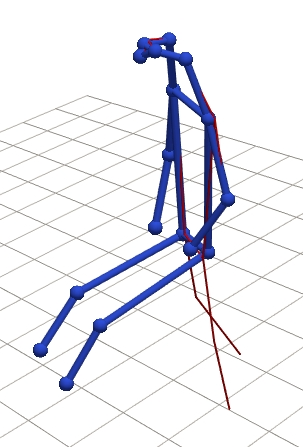
\includegraphics[width=\linewidth]{figures/qualitative1.png}
    \caption{Partially occluded person.}
    \label{fig:qual-occlusion}
  \end{subfigure}
  \hfill
  \begin{subfigure}[t]{0.19\linewidth}
    \centering
    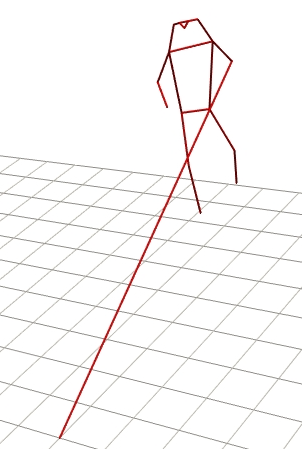
\includegraphics[width=\linewidth]{figures/qualitative2.png}
    \caption{Inactive track seen by only one camera.}
    \label{fig:qual-single}
  \end{subfigure}
  \hfill
  \begin{subfigure}[t]{0.19\linewidth}
    \centering
    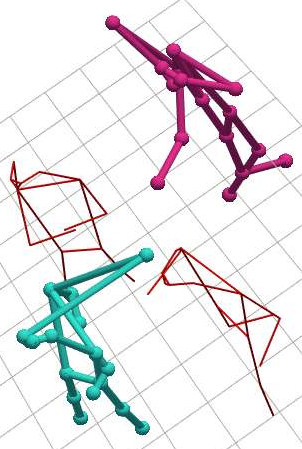
\includegraphics[width=\linewidth]{figures/qualitative3.png}
    \caption{Active track seen by only one camera.}
    \label{fig:qual-single2}
  \end{subfigure}
  \hfill
  \begin{subfigure}[t]{0.19\linewidth}
    \centering
    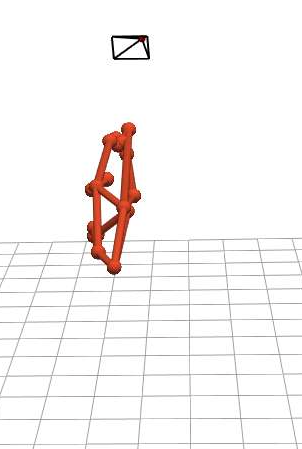
\includegraphics[width=\linewidth]{figures/qualitative4.png}
    \caption{Detection of person while exiting.}
    \label{fig:qual-leave}
  \end{subfigure}
  \hfill
  \caption{Some qualitative samples extracted from the evaluation results on the test set that exhibit commonly seen issues with the tracking system. Ground truth skeletons are drawn using thing red lines, while predicted skeletons are drawn thicker and with different colors per track.}
  \label{fig:qual}
\end{figure*}

\subsection{Quantitative Results} \label{quant}

Quantitative results for the system on the chosen test sequences can be found in \cref{fig:eval-results}. When keeping the model fixed to YOLO26n-pose and increasing the number of cameras from 4 to 16, a significant reduction in pose and localization errors can be observed. The joint position error decreases drastically by about half, from 5.439 cm down to 2.576 cm. This indicates that incorporating more viewpoints substantially improves 3D localization and pose estimation accuracy. Also, the increase in camera views brings improvements in recall. Recall increases from 0.975 with 4 cameras to 0.998 when using 16 cameras, indicating fewer missed detections likely because the cameras now cover more angles that would otherwise not be visible. There exists a slight trade-off in tracking accuracy and precision. Adding more cameras leads to a decrease in precision from 0.966 for 4 cameras to 0.955 with 16. This can be explained by the fact that more camera views introduce a higher likelihood of false positives and could also indicate limitations in the association algorithm. MOTA hits a sweet spot of 0.960 with 8 cameras. 

In contrast, when keeping the camera count fixed at 4 and scaling up the model complexity from YOLO26n-pose to YOLO26l-pose, we see improvements in all metrics. The largest model achieves the best overall MOTA of 0.960 and precision of 0.977. Upgrading the model capacity also reduces MPJPE from 5.439 cm to 4.554 cm. However, the improvement in this metric is not as significant as with the addition of more cameras.

Finally, \cref{fig:eval-by-scene} shows the average performance per scene across performed evaluations. It can be seen that the \inlinecode{160224_haggling1} scene is the one with the lowest performance metrics. In this scene, MOTA and Precision suffer from a large increase in false positives. This scene contains the most entries and exists from the room as well as more close contact, which the tracking algorithm can struggle with. The system performs particularly well on \inlinecode{161029_piano4} and \inlinecode{170915_office1}. This is largely because in these scenes the persons are in the room for the entire duration of the video sequence, avoiding a big source of errors for the system.


\subsection{Qualitative Results} \label{qual}

Some qualitative evaluation has also been performed for this project.

\subsubsection{Impact of the Skeletal Constraints}

% TODO add another figure with SALSA
% TODO add another figure with Covision data
% TODO talk about impact of the skeletal constraints

\subsubsection{Common Failure Modes}

% TODO mention that some if the failure modes are solved by the skeletal constraints
The results of the system on the tests sequences has been visualized and a number of common issues have been identified. Some examples of these failure modes are shown in \cref{fig:qual}.

\paragraph{Partially Occluded Person}
One very common failure mode is depicted in \cref{fig:qual-occlusion}. When a person is partially occluded in all camera views, then the position of the unobserved keypoints tends to shift in unnatural ways, as can be seen with the legs keypoints in the given example. This problem is made worse by the fact that the YOLO model tend to predict invisible keypoints in unnatural positions, and while their visibility score is low, it can still commutatively have a significant effect over multiple frames. This issue causes increased joint position errors.

\paragraph{Inactive Track Seen by Only One Camera}
Another commonly observed failure is shown in \cref{fig:qual-single}. When a person first enters the room, typically only one camera can see them. This means that it is not possible to create a new track for that person. This causes false positives, and therefore reduced MOTA and Recall, whenever a person enters the room.

% TODO mention that this is less of a problem with the skeletal constraints
\paragraph{Active Track Seen by Only One Camera}
\Cref{fig:qual-single2} shows another issue that can occur when only a single camera is able to see a given person. In this case, the track has already been initialized, but the person has moved into a location where they are no longer seen by two cameras. In this case the depth coordinate from the camera can drift as the person moves, causing distorted skeletons before and behind the actual ground truth.

\paragraph{Detection of Person While Exiting}
\Cref{fig:qual-leave} show a failure that occurs when a person leaves the room. In this case, the camera that is pointing at the exit will see the person for longer than the actual ground truth indicates. This causes false positives and therefore worse MOTA and Precision. Note that in this case we also have the above mention issue of an active track seen by only one camera.
